\documentclass[fleqn,12pt]{llncs}

\usepackage[hidelinks]{hyperref}
\usepackage {mathpartir}
\usepackage {graphicx}
\usepackage{bigpage}
\usepackage{bcprules}
\usepackage{amsmath}
\usepackage{amssymb}
\usepackage{amsfonts}
\usepackage{amstext}
\usepackage{latexsym}
\usepackage{longtable}
\usepackage{stmaryrd}
%% \usepackage[T1]{fontenc}
%% \usepackage[utf8]{inputenc}
%% \usepackage[normalem]{ulem}
\usepackage[svgnames]{xcolor}
%\usepackage[paperheight=27.94cm,paperwidth=21.59cm,left=2.54cm,right=2.54cm,top=2.54cm,bottom=2.54cm]{geometry}
\usepackage {graphicx}
\usepackage{color}


%\setlength\parindent{0pt}
\renewcommand{\arraystretch}{1.3}

% Double brackets
\newcommand{\ldb}{[\![}
\newcommand{\rdb}{]\!]}
\newcommand{\ldrb}{(\!(}
\newcommand{\rdrb}{)\!)}
\newcommand{\lrbb}{(\!|}
\newcommand{\rrbb}{|\!)}
\newcommand{\lliftb}{\langle\!|}
\newcommand{\rliftb}{|\!\rangle}
\newcommand{\lrcb}{\{\!\!\{}
\newcommand{\rrcb}{\}\!\!\}}
%\newcommand{\plogp}{:\!-}
\newcommand{\plogp}{\leftarrow}
%\newcommand{\plogp}{\coloneq}
% \newcommand{\lpquote}{\langle}
% \newcommand{\rpquote}{\rangle}
% \newcommand{\lpquote}{\lceil}
% \newcommand{\rpquote}{\rceil}
\newcommand{\lpquote}{\ulcorner}
\newcommand{\rpquote}{\urcorner}
\newcommand{\newkw}{\nu}

% SYNTAX
\newcommand{\id}[1]{\texttt{#1}}
\newcommand{\none}{\emptyset}
\newcommand{\eps}{\epsilon}
\newcommand{\set}[1]{\{#1\}}
\newcommand{\rep}[2]{\id{\{$#1$,$#2$\}}}
\newcommand{\elt}[2]{\id{$#1$[$#2$]}}
\newcommand{\infinity}{$\infty$}

\newcommand{\pzero}{\mathsf{0}}
\newcommand{\seq}{\mathsf{\id{,}}}
\newcommand{\all}{\mathsf{\id{\&}}}
\newcommand{\choice}{\mathsf{\id{|}}}
\newcommand{\altern}{\mathsf{\id{+}}}
\newcommand{\juxtap}{\mathsf{\id{|}}}
\newcommand{\concat}{\mathsf{.}}
\newcommand{\punify}{\mathsf{\id{:=:}}}
\newcommand{\fuse}{\mathsf{\id{=}}}
\newcommand{\scong}{\mathsf{\equiv}}
\newcommand{\nameeq}{\mathsf{\equiv_N}}
\newcommand{\alphaeq}{\mathsf{\equiv_{\alpha}}}
\newcommand{\arrvec}[1]{\overrightarrow{#1}}
\newcommand{\names}[1]{\mathsf{N}(#1)}
\newcommand{\freenames}[1]{\mathsf{FN}(#1)}
\newcommand{\boundnames}[1]{\mathsf{BN}(#1)}
%\newcommand{\lift}[2]{\texttt{lift} \; #1 \concat #2}
\newcommand{\binpar}[2]{#1 \mathsf{|} #2}
\newcommand{\binparx}[2]{\mathsf{par}(#1, #2)}
\newcommand{\binpart}[2]{\mathbf{par}(\mathbf{#1}, \mathbf{#2})}
\newcommand{\binpartl}[2]{\mathbf{par}_{L}(\mathbf{#1}, \mathbf{#2})}
\newcommand{\binpartr}[2]{\mathbf{par}_{R}(\mathbf{#1}, \mathbf{#2})}
\newcommand{\outputp}[2]{#1\mathsf{!}(#2)}
\newcommand{\outputt}[2]{\mathbf{#1}\mathsf{!}(\mathbf{#2})}
\newcommand{\prefix}[3]{\mathsf{for(}#2 \leftarrow #1 \mathsf{)} #3}
\newcommand{\prefixt}[3]{\mathbf{for}\mathbf{(}\mathbf{#2} \leftarrow \mathbf{#1} \mathbf{)} \mathbf{#3}}
%%\newcommand{\lift}[2]{#1 \lliftb #2 \rliftb}
\newcommand{\lift}[2]{#1 \mathsf{!}(#2)}
\newcommand{\clift}[1]{\lliftb #1 \rliftb}
\newcommand{\quotep}[1]{\mathsf{@} #1}
\newcommand{\quotet}[1]{\mathbf{@} \mathbf{#1}}
\newcommand{\dropn}[1]{\mathsf{*} #1}
\newcommand{\dropt}[1]{\mathbf{*} \mathbf{#1}}
\newcommand{\procn}[1]{\stackrel{\cdot}{#1}}
\newcommand{\commr}[4]{\mathsf{comm(}#1, #2, #3, #4  \mathsf{)}}
\newcommand{\commt}[3]{\mathbf{comm(}\mathbf{#1}, \mathbf{#2}, \mathbf{#3} \mathbf{)}}

\newcommand{\newp}[2]{(\newkw \; #1 ) #2}
\newcommand{\bangp}[1]{! #1}

\newcommand{\substp}[2]{\{ \quotep{#1} / \quotep{#2} \}}
\newcommand{\substn}[2]{\{ #1 / #2 \}}
\newcommand{\msubstn}[2]{\lrcb #1 / #2 \rrcb}

\newcommand{\psubstp}[2]{\widehat{\substp{#1}{#2}}}
\newcommand{\psubstn}[2]{\widehat{\substn{#1}{#2}}}

\newcommand{\applyp}[2]{#1 \langle #2 \rangle}
\newcommand{\absp}[2]{( #1 ) #2}
\newcommand{\annihilate}[1]{#1^{\times}}
\newcommand{\dualize}[1]{#1^{\bullet}}
\newcommand{\ketp}[1]{\mathsf{|}#1 \rangle}
\newcommand{\brap}[1]{\langle #1 \mathsf{|}}
\newcommand{\testp}[2]{\langle #1 \mathsf{|} #2 \rangle}
\newcommand{\testnp}[3]{\langle #1 \mathsf{|} #2 \mathsf{|} #3 \rangle}

\newcommand{\transitions}[3]{\mathbin{#1 \stackrel{#2}{\longrightarrow} #3}}
\newcommand{\meaningof}[1]{\ldb #1 \rdb}
\newcommand{\pmeaningof}[1]{\ldb #1 \rdb}
\newcommand{\nmeaningof}[1]{\lrbb #1 \rrbb}

\newcommand{\Proc}{\mathsf{Proc}}
\newcommand{\QProc}{\quotep{\mathsf{Proc}}}
\newcommand{\MixSumProc}{\mathsf{MixSumProc}}

\newcommand{\entailm}{\mathbin{\vdash_{\mathfrak m}}} %matching
\newcommand{\entailp}{\mathbin{\vdash_{\mathfrak p}}} %behavioral
\newcommand{\entailv}{\mathbin{\vdash_{\mathfrak v}}} %validation
\newcommand{\congd}{\mathbin{\equiv_{\mathfrak d}}}
\newcommand{\congs}{\mathbin{\equiv_{\mathfrak s}}}
\newcommand{\congp}{\mathbin{\equiv_{\mathfrak p}}}
%\newcommand{\logequiv}{\mathbin{\leftrightarrow}}

\newcommand{\barb}[2]{\mathbin{#1 \downarrow_{#2}}}
\newcommand{\dbarb}[2]{\mathbin{#1 \Downarrow_{#2}}}

% From pi-duce paper
\newcommand{\red}{\rightarrow}
\newcommand{\wred}{\Rightarrow}
\newcommand{\redhat}{\hat{\longrightarrow}}
\newcommand{\lred}[1]{\stackrel{#1}{\longrightarrow}} %transitions
\newcommand{\wlred}[1]{\stackrel{#1}{\Longrightarrow}}

\newcommand{\opm}[2]{\overline{#1} [ #2 ]} % monadic
\newcommand{\ipm}[2]{{#1} ( #2 )} 
\newcommand{\ipmv}[2]{{#1} ( #2 )} % monadic
\newcommand{\parop}{\;|\;}		% parallel operator
\newcommand{\patmatch}[3]{#2 \in #3 \Rightarrow #1}
\newcommand{\sdot}{\, . \,}		% Space around '.'
\newcommand{\bang}{!\,}
%\newcommand{\fuse}[1]{\langle #1 \rangle}		
\newcommand{\fusion}[2]{#1 = #2} % fusion prefix/action
\newcommand{\rec}[2]{\mbox{\textsf{rec}} \, #1. \, #2}
\newcommand{\match}[2]{\mbox{\textsf{match}} \; #1 \; \mbox{\textsf{with}} \; #2}
\newcommand{\sep}{:}
\newcommand{\val}[2]{\mbox{\textsf{val}} \; #1 \; \mbox{\textsf{as}} \; #2}

\newcommand{\rel}[1]{\;{\mathcal #1}\;} %relation
\newcommand{\bisim}{\stackrel{.}{\sim}_b} %bisimilar
\newcommand{\wb}{\approx_b} %weak bisimilar
\newcommand{\bbisim}{\stackrel{\centerdot}{\sim}} %barbed bisimilar
\newcommand{\wbbisim}{\stackrel{\centerdot}{\approx}} %weak barbed bisimilar
\newcommand{\bxless}{\lesssim}	%expansion less (amssymb required)
\newcommand{\bxgtr}{\gtrsim}	%expansion greater (amssymb required)
\newcommand{\beq}{\sim}		%barbed congruent
\newcommand{\fwbeq}{\stackrel{\circ}{\approx}}	%weak barbed congruent
\newcommand{\wbeq}{\approx}	%weak barbed congruent
\newcommand{\sheq}{\simeq}	%symbolic hypereq
\newcommand{\wbc}{\approx_{cb}}

% rho logic

\newcommand{\ptrue}{\mathbin{true}}
\newcommand{\psatisfies}[2]{#1 \models #2}
\newcommand{\pdropf}[1]{\rpquote #1 \lpquote}
\newcommand{\plift}[2]{#1 \lliftb #2 \rliftb}
\newcommand{\pprefix}[3]{\langle #1 ? #2 \rangle #3}
\newcommand{\pgfp}[2]{\textsf{rec} \; #1 \mathbin{.} #2}
\newcommand{\pquant}[3]{\forall #1 \mathbin{:} #2 \mathbin{.} #3}
\newcommand{\pquantuntyped}[2]{\forall #1 \mathbin{.} #2}
\newcommand{\riff}{\Leftrightarrow}

\newcommand{\PFormula}{\mathbin{PForm}}
\newcommand{\QFormula}{\mathbin{QForm}}
\newcommand{\PropVar}{\mathbin{\mathcal{V}}}

% qm notation
\newcommand{\state}[1]{\juxtap #1 \rangle}
\newcommand{\event}[1]{\langle #1 \juxtap}
\newcommand{\innerprod}[2]{\langle #1 \juxtap #2 \rangle}
\newcommand{\prmatrix}[2]{\juxtap #1 \rangle \langle #2 \juxtap}
\newcommand{\fprmatrix}[3]{\juxtap #1 \rangle #2 \langle #3 \juxtap}

% End piduce contribution

\newcommand{\typedby}{\mathbin{\:\colon}}
\newcommand{\mixedgroup}[1]{\id{mixed($#1$)}}
\newcommand{\cast}[2]{\id{CAST AS} \; #1 \; (#2)}
\newcommand{\bslsh}{\mathbin{\id{\\}}}
\newcommand{\bslshslsh}{\mathbin{\id{\\\\}}}
\newcommand{\fslsh}{\mathbin{\id{/}}}
\newcommand{\fslshslsh}{\mathbin{\id{//}}}
\newcommand{\bb}[1]{\mbox{#1}}
\newcommand{\bc}{\mathbin{\mathbf{::=}}}
\newcommand{\bm}{\mathbin{\mathbf\mid}}
%\newcommand{\bm}{\mathbin{\mathbf\mid}}
\newcommand{\be}{\mathbin{=}}
\newcommand{\bd}{\mathbin{\buildrel {\rm \scriptscriptstyle def} \over \be}}
%\newcommand{\category}[1]{\mbox{\bf #1}}

%GRAMMAR
\newlength{\ltext}
\newlength{\lmath}
\newlength{\cmath}
\newlength{\rmath}
\newlength{\rtext}

\settowidth{\ltext}{complex type name}
\settowidth{\lmath}{$xxx$}
\settowidth{\cmath}{$::=$}
\settowidth{\rmath}{\id{attributeGroup}}
\settowidth{\rtext}{repetition of $g$ between $m$ and $n$ times}

\newenvironment{grammar}{
  \[
  \begin{array}{l@{\quad}rcl@{\quad}l}
  \hspace{\ltext} & \hspace{\lmath} & \hspace{\cmath} & \hspace{\rmath} & \hspace{\rtext} \\
}{
  \end{array}\]
}

% Over-full v-boxes on even pages are due to the \v{c} in author's name
%\vfuzz2pt % Don't report over-full v-boxes if over-edge is small

% THEOREM Environments ---------------------------------------------------
% MATH -------------------------------------------------------------------
 \newcommand{\veps}{\varepsilon}
 \newcommand{\To}{\longrightarrow}
 \newcommand{\h}{\mathcal{H}}
 \newcommand{\s}{\mathcal{S}}
 \newcommand{\A}{\mathcal{A}}
 \newcommand{\J}{\mathcal{J}}
 \newcommand{\M}{\mathcal{M}}
 \newcommand{\W}{\mathcal{W}}
 \newcommand{\X}{\mathcal{X}}
 \newcommand{\BOP}{\mathbf{B}}
 \newcommand{\BH}{\mathbf{B}(\mathcal{H})}
 \newcommand{\KH}{\mathcal{K}(\mathcal{H})}
 \newcommand{\Real}{\mathbb{R}}
 \newcommand{\Complex}{\mathbb{C}}
 \newcommand{\Field}{\mathbb{F}}
 \newcommand{\RPlus}{\Real^{+}}
 \newcommand{\Polar}{\mathcal{P}_{\s}}
 \newcommand{\Poly}{\mathcal{P}(E)}
 \newcommand{\EssD}{\mathcal{D}}
 \newcommand{\Lom}{\mathcal{L}}
 \newcommand{\States}{\mathcal{T}}
 \newcommand{\abs}[1]{\left\vert#1\right\vert}
% \newcommand{\set}[1]{\left\{#1\right\}}
%\newcommand{\seq}[1]{\left<#1\right>}
 \newcommand{\norm}[1]{\left\Vert#1\right\Vert}
 \newcommand{\essnorm}[1]{\norm{#1}_{\ess}}

%%% NAMES
\newcommand{\Names}{{\mathcal N}}
\newcommand{\Channels}{{\sf X}}
\newcommand{\Variables}{{\mathcal V}}
\newcommand{\Enames}{{\mathcal E}}
\newcommand{\Nonterminals}{{\mathcal S}}
\newcommand{\Pnames}{{\mathcal P}}
\newcommand{\Dnames}{{\mathcal D}}
\newcommand{\Types}{{\mathcal T}}

\newcommand{\fcalc}{fusion calculus}
\newcommand{\xcalc}{${\mathfrak x}$-calculus}
\newcommand{\lcalc}{$\lambda$-calculus}
\newcommand{\pic}{$\pi$-calculus}
\newcommand{\spic}{spi-calculus}
\newcommand{\rhoc}{$\rho$-calculus}
\newcommand{\rhol}{$\rho$-logic}
\newcommand{\hcalc}{highwire calculus}
\newcommand{\dcalc}{data calculus}
%XML should be all caps, not small caps. --cb
%\newcommand{\xml}{\textsc{xml}}
\newcommand{\xml}{XML} 
\newcommand{\Opp}[1]{\mathsf{#1}^{\mathsf{op}}}
 

\begin{document}
\def\lastname{Meredith}

\title{Meta-MeTTa: an operational semantics for MeTTa}
\titlerunning{meta-metta}

\date{2 March 2023}

\author{ Lucius Gregory Meredith\inst{1} \\
         \and 
         Ben Goertzel\inst{2}
         \and Jonathan Warrell\inst{3}
}
\institute{
        {CEO, F1R3FLY.io 9336 California Ave SW, Seattle, WA 98103, USA} \\
  \email{ f1r3fly.ceo.com } \\
  \and
  {CEO, SingularityNet} \\
  \email{ ben@singularitynet.io } \\
  \and
  {Researcher, SingularityNet} \\
  \email{jonathan.warrell@singularitynet.io}
}
 

\maketitle              % typeset the title of the contribution

%%% ----------------------------------------------------------------------

\begin{abstract}

  We present an operational semantics for the language MeTTa.

\end{abstract}

%\keywords{Process calculi, knots, invariants}

% \begin{keyword}
% concurrency, message-passing, process calculus, reflection, program logic
% \end{keyword}

%\end{frontmatter}


\section{Introduction and motivation}
We present the operational semantics for the language MeTTa. MeTTa is designed as a language in which humans and AGIs write the behavior of AGIs, being jointly developed by SingularityNet.io and F1R3FLY.io, as part of SingularityNet.io's OpenCog and Hyperon projects \cite{DBLP:conf/agi/HartG08} \cite{YT:GoertzelIklePotapovHyperon2022}. One of the principle motivations of this document is to help developers of MeTTa clients know what is a correct and compliant implementation. The document serves roughly the same function as the JVM specification or Ethereum's Yellow paper \cite{wood2014ethereum}.


\section{Towards a common language for computational dynamics}
Three of the most successful branches of scientific discourse all agree on the shape of a model adequate for expressing and effecting computation. Physics, computer science, and mathematics all use the same standard shape. A model adequate for computation comes with an algebra of states and “laws of motion.”

One paradigmatic example from physics is Hilbert spaces and the Schroedinger equation. In computer science and mathematics the algebra of states is further broken down into a monad (the free algebra of states) and an algebra of the monad recorded as some equations on the free algebra.

Computer science represents laws of motion, aka state transitions, as rewrite rules exploiting the structure of states to determine transitions to new states. Mainstream mathematics is a more recognizable generalization of physics, coding state transitions, aka behavior, via morphisms (including automorphisms) between state spaces.

But all three agree to a high degree of specificity on what ingredients go into a formal presentation adequate for effecting computation.

\subsection{Examples from computer science}
Since Milner's seminal Functions as processes paper, the gold standard for a presentation of an operational semantics is to present the algebra of states via a grammar (a monad) and a structural congruence (an algebra of the monad), and the rewrite rules in Plotkin-style SOS format.

\subsubsection{$\lambda$-calculus}

\paragraph{Algebra of States}
\begin{eqnarray*}
  Term[V] & \bc & V \\
  & \;\bm\; & \lambda V.Term[V] \\
  & \;\bm\; & \mathsf{(} Term[V] \; Term[V] \mathsf{)}
\end{eqnarray*}

The structural congruence is the usual $\alpha$-equivalence, namely that $\lambda x.M \scong \lambda y.(M\{y / x\})$ when $y$ not free in $M$.

It is evident that $Term[V]$ is a monad and imposing $\alpha$-equivalence gives an algebra of the monad.

\paragraph{Transitions}
The rewrite rule is the well know $\beta$-reduction.
\begin{mathpar}
  \inferrule* [lab=Beta]{}{((\lambda x.M)N) \to M\{N / x\}}
\end{mathpar}

\subsubsection{$\pi$-calculus}

\paragraph{Algebra of States}
\begin{eqnarray*}
  Term[N] & \bc & \mathsf{0} \\
  & \;\bm\; & \mathsf{for}\mathsf{(}N \leftarrow N\mathsf{)}Term[N] \\
  & \;\bm\; & N\mathsf{!}\mathsf{(}N\mathsf{)} \\
  & \;\bm\; & \mathsf{(}\mathsf{new}\; N\mathsf{)}Term[N] \\
  & \;\bm\; & Term[N] \; \mathsf{|}\; Term[N] \\
  & \;\bm\; & \mathsf{!}Term[N]
\end{eqnarray*}

The structural congruence is the smallest equivalence relation including $\alpha$-equivalence making $(Term[N],\;\mathsf{|}\;,\mathsf{0})$ a commutative monoid, and respecting

\begin{eqnarray*}
  \mathsf{(}\mathsf{new}\; x\mathsf{)}\mathsf{(}\mathsf{new}\; x\mathsf{)}P & \scong & \mathsf{(}\mathsf{new}\; x\mathsf{)}P \\
  \mathsf{(}\mathsf{new}\; x\mathsf{)}\mathsf{(}\mathsf{new}\; y\mathsf{)}P & \scong & \mathsf{(}\mathsf{new}\; y\mathsf{)}\mathsf{(}\mathsf{new}\; x\mathsf{)}P \\
  (\mathsf{(}\mathsf{new}\; x\mathsf{)}P)\mathsf{|}Q & \scong & \mathsf{(}\mathsf{new}\; x\mathsf{)}(P\mathsf{|}Q), x \notin \freenames{Q}
\end{eqnarray*}

Again, it is evident that $Term[N]$ is a monad and imposing the structural congruence gives an algebra of the monad.

\paragraph{Transitions}
The rewrite rules divide into a core rule, and when rewrites apply in
context.
\begin{mathpar}
  \inferrule* [lab=COMM]{}{\mathsf{for}\mathsf{(}y \leftarrow x\mathsf{)}P \mathsf{|} x\mathsf{!}\mathsf{(}z\mathsf{)} \to P\{ z / y \}} \\
  \and  
  \inferrule* [lab=PAR]{P \to P'}{(\mathsf{new}\; x)P \to (\mathsf{new}\; x)P'}
  \and  
  \inferrule* [lab=PAR]{P \to P'}{P\mathsf{|}Q \to P'\mathsf{|}Q} \\
  \and
  \inferrule* [lab=STRUCT]{P \scong P' \to Q' \scong Q}{P \to Q}
\end{mathpar}

\subsubsection{rho-calculus}

\paragraph{Algebra of States}
Note that the rho-calculus is different from the $\lambda$-calculus and the $\pi$-calculus because it is \emph{not} dependent on a type of variables or names. However, it does give us the opportunity to expose how ground types, such as Booleans, numeric and string operations are imported into the calculus. The calculus does depend on the notion of a $0$ process. In fact, this could be any builtin functionality. The language rholang, derived from the rho-calculus, imports all literals as \emph{processes}. Note that this is in the spirit of the $\lambda$-calculus and languages derived from it: Booleans, numbers, and strings are terms, on the level with $\lambda$ terms.

So, the parameter to the monad for the rho-calculus takes the collection of builtin processes. Naturally, for all builtin processes other than $0$ there have to be reduction rules. For brevity, we take $Z = \{0\}$.
\begin{mathpar}
\inferrule* [lab=process] {} {Term[Z] \bc Z \;\bm\; \mathsf{for}(
  Name[Z] \leftarrow Name[Z] )Term[Z] \;\bm\; Name[Z]\mathsf{!}(Term[Z]) 
  \\ \and \;\bm\; \mathsf{*}Name[Z] \;\bm\; Term[Z]\mathsf{|}Term[Z] } \\
\and \inferrule* [lab=name] {}
     {Name[Z] \bc \mathsf{@}Term[Z] }
\end{mathpar}

The structural congruence is the smallest equivalence relation including $\alpha$-equivalence making $(P,\;\mathsf{|}\;,\mathsf{0})$ a commutative monoid.

Again, it is evident that $Term[Z]$ is a monad and imposing the structural congruence gives an algebra of the monad.

\paragraph{Transitions}
The rewrite rules divide into a core rule, and when rewrites apply in
context.
\begin{mathpar}
  \inferrule* [lab=COMM] {x_{t} \;\nameeq\; x_{s}} {\mathsf{for}(y \leftarrow x_{t} )P \;\mathsf{|}\; x_{s}!(Q)
  \red P\substn{\quotep{Q}}{y}} \\
  \and
  \inferrule* [lab=PAR]{P \red P'}{P\mathsf{|}Q \red P'\mathsf{|}Q}
  \and
  \inferrule* [lab=STRUCT]{{P \;\scong\; P'} \andalso {P' \red Q'} \andalso {Q' \;\scong\; Q}}{P \red Q}
\end{mathpar}

\pagebreak
\subsubsection{The JVM}

While its complexity far exceeds the presentations above, the JVM specification respects this same shape. Here is an example from the specification of what the operation aaload does.

\begin{figure}[h!]
  \scalebox{0.75}{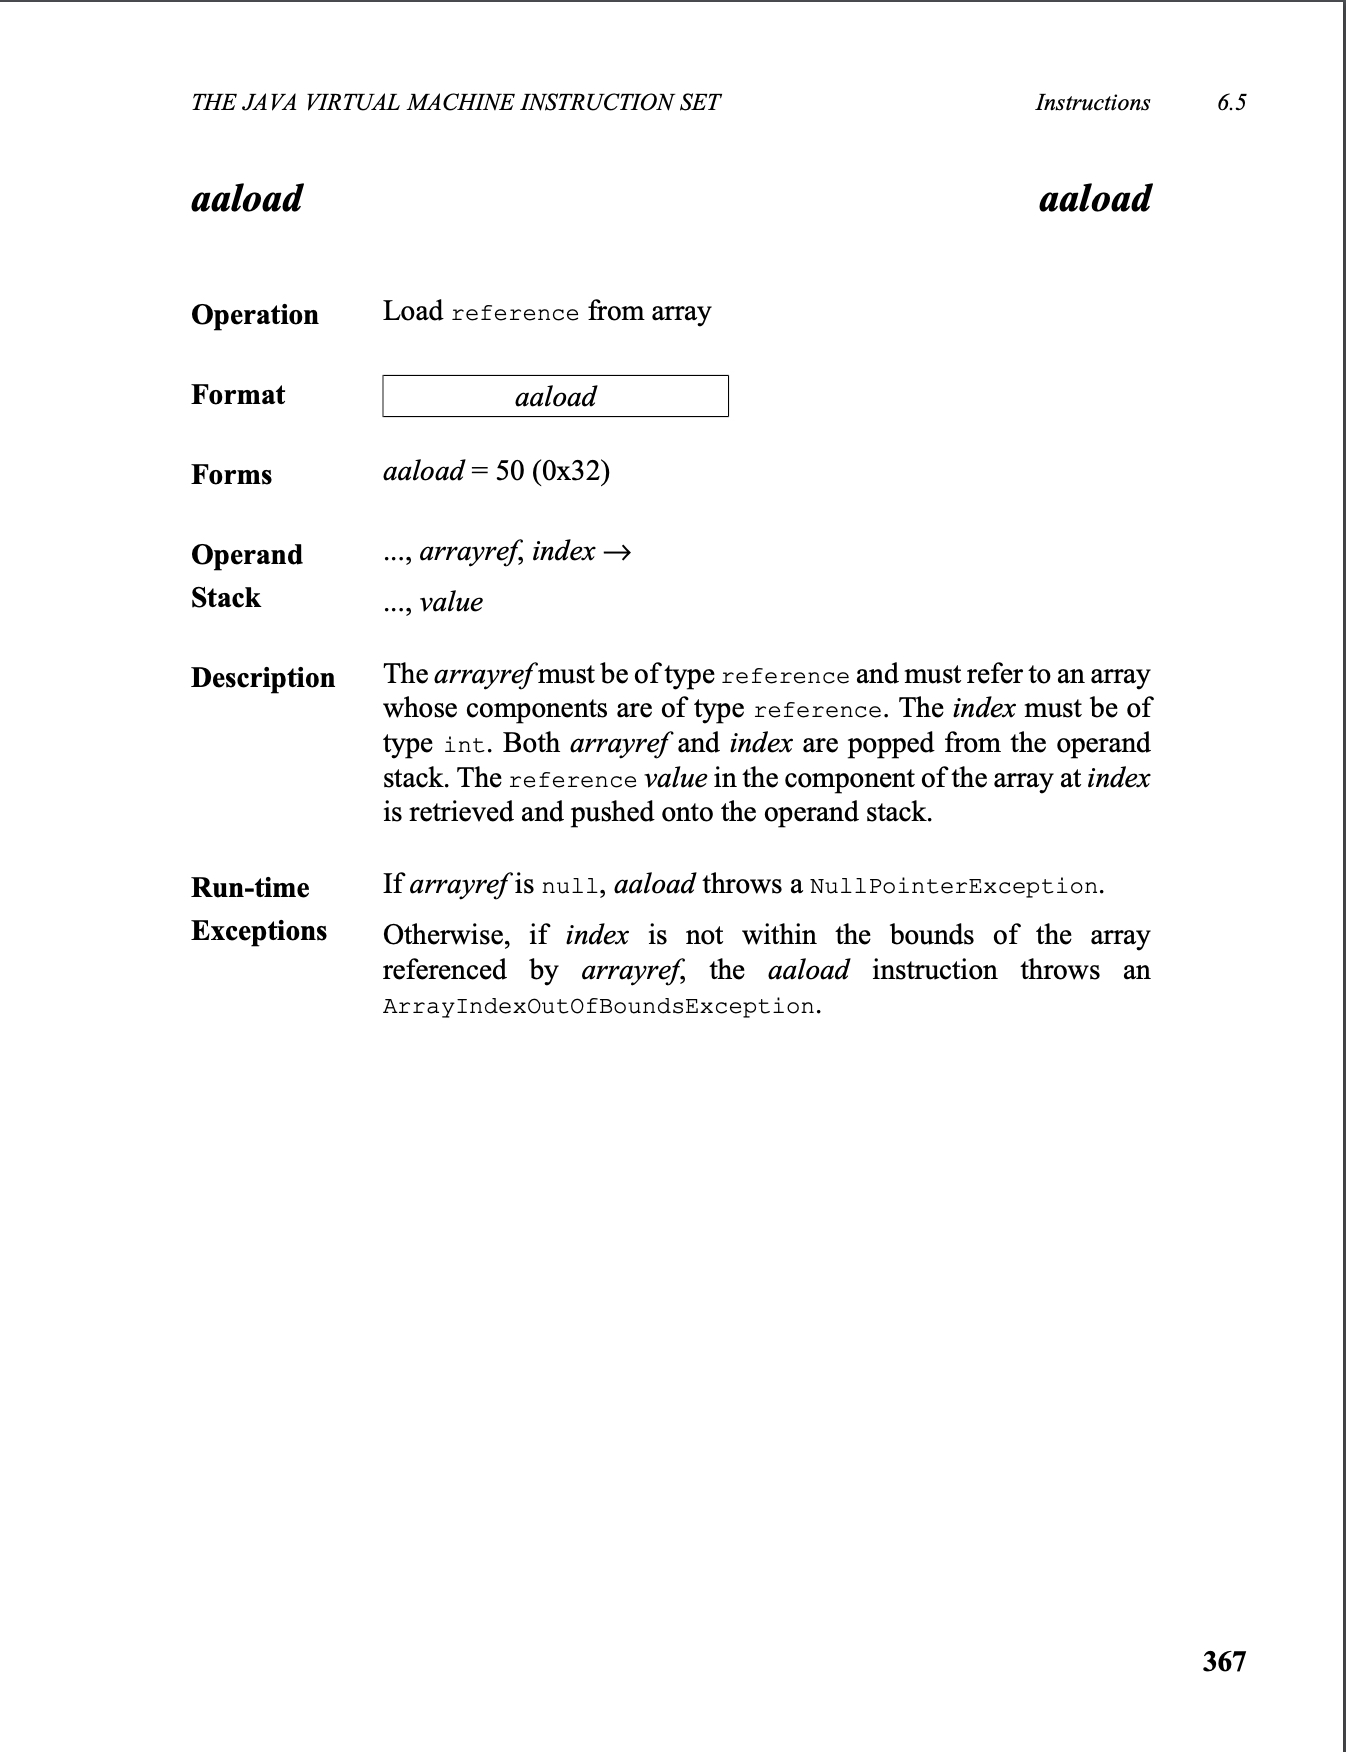
\includegraphics[width=\linewidth]{JVMSpecAALOAD.jpg}}
  \caption{AALOAD instruction specification}
  \label{fig:AALOADSpec}
\end{figure}

\paragraph{WYSIWYG semantics}One important point about the JVM versus the previous three
examples. The first three examples are examples of WYSIWYG operational
semantics in the sense that the states \emph{are} the terms of the
calculi. In the case of the JVM the terms in the language are only
part of the state, which includes the stack, the heap, and several
registers. WYSIWYG models make static analysis dramatically
simpler. Specifically, an analyzer only has to look at terms in the
language.


\section{A presentation of the semantics of MeTTa}

A presentation of the semantics of MeTTa must therefore provide a monad describing the algebra of states, a structural equivalence quotienting the algebra of states, and some rewrite rules describing state transitions. Such a description is the minimal description that meets the standard for describing models of computation. 


Note that to present such a description requires at least that much expressive power in the system used to formalize the presentation. That is, the system used to present a model of computation is itself a model of computation admitting a presentation in terms of an algebra of states and some rewrites. This is why a meta-circular evaluator is a perfectly legitimate presentation. That is, a presentation of MeTTa’s semantics in MeTTa is perfectly legitimate. Meta-circular presentations are more difficult to unpack, which is why such presentations are typically eschewed, but they are admissible. In fact, a meta-circular evaluator may be the most pure form of presentation.


But, this fact has an important consequence. No model that is at least Turing complete can be “lower level” than any other.

\subsection{Rationale for such a presentation}

The rationale for such a presentation is not simply that this is the way it’s done. Instead, the benefits include

\begin{itemize}
  \item an effective (if undecidable) notion of program equality;
  \item an independent specification allowing implementations;
  \item meta-level computation, including type checking, model checking, macros, computational reflection, etc.
\end{itemize}

\subsection{MeTTa Operational Semantics}
The complexity of MeTTa's operational semantics is somewhere between the simplicity of the $\lambda$-calculus and the enormity of the JVM.

\subsubsection{Algebra of States}

%% Non-terminals are enclosed between $<$ and $>$. 
%% The symbols -$>$ (production),  \textbf{$|$}  (union) 
%% and \textbf{eps} (empty rule) belong to the BNF notation. 
%% All other symbols are terminals.

\paragraph{Terms}
\begin{eqnarray*}
  Term & \bc & \mathsf{(} Term \; [Term] \mathsf{)} \\
  & \;\bm\; & \mathsf{\{} Term \; [Term] \mathsf{\}} \\
  & \;\bm\; & \mathsf{(} Term{} \;\mathsf{|}\; [Receipt] \; \mathsf{.} \; [Term] \mathsf{)} \\
  & \;\bm\; & \mathsf{\{} Term \;\mathsf{|}\; [Receipt] \; \mathsf{.} \; [Term] \mathsf{\}} \\
& \;\bm\; & Atom
\end{eqnarray*}

We impose the equation $\mathsf{\{} \ldots, t, u, \ldots \mathsf{\}} = \mathsf{\{} \ldots, u, t, \ldots \mathsf{\}}$, making terms of this form multisets. Note that for multiset comprehensions this amounts to non-determinism in the order of the terms delivered, but they are still streams. We use $\mathsf{\{}Term\mathsf{\}}$ to denote the set of terms that are (extensionally or intensionally) defined multisets, and $\mathsf{(}Term\mathsf{)}$ to denote the set of terms that are (extensionally or intensionally) defined lists.

We assume a number of polymorphic operators, such as $\pplus$ which acts as union on multisets and append on lists and concatenation on strings, and $::$ which acts as cons on lists and the appropriate generalization for the other data types.

\paragraph{Term sequences}
\begin{eqnarray*}
  [Term] & \bc & \epsilon \\
  & \;\bm \; & Term \\
  & \;\bm \; & Term \; [Term]
\end{eqnarray*}

\paragraph{Bindings}
\begin{eqnarray*}
  Receipt & \bc & ReceiptLinearImpl \\
  & \;\bm \; & ReceiptRepeatedImpl \\
  & \;\bm \; & ReceiptPeekImpl
\end{eqnarray*}
\begin{eqnarray*}
  [Receipt] & \bc & Receipt \\
  & \;\bm \; & Receipt \mathsf{;}\; [Receipt]
\end{eqnarray*}
\begin{eqnarray*}
  ReceiptLinearImpl & \bc & [LinearBind] \\
  LinearBind & \bc & [Name] \; NameRemainder \; \mathsf{\leftarrow} \; AtomSource
\end{eqnarray*}
\begin{eqnarray*}
  [LinearBind] & \bc & LinearBind \\
  & \;\bm \; & LinearBind \;\mathsf{\&}\; [LinearBind]
\end{eqnarray*}
\begin{eqnarray*}
  AtomSource & \bc & Name \\
  & \;\bm \; & Name \mathsf{?!} \\
  & \;\bm \; & Name \mathsf{!?} \mathsf{(} [Term] \mathsf{)} \\
  ReceiptRepeatedImpl & \bc & [RepeatedBind] \\
  RepeatedBind & \bc & [Name] \; NameRemainder \; \mathsf{\Leftarrow} \; Atom
\end{eqnarray*}
\begin{eqnarray*}
  [RepeatedBind] & \bc & RepeatedBind \\
  & \;\bm \; & RepeatedBind \; \mathsf{\&}\; [RepeatedBind] \\
  ReceiptPeekImpl & \bc & [PeekBind] \\
  PeekBind & \bc & [Name] \; NameRemainder \; \mathsf{\leftharpoonup}\; Atom
\end{eqnarray*}
\begin{eqnarray*}
  [PeekBind] & \bc & PeekBind \\
  & \;\bm \; & PeekBind \; \mathsf{\&}\; [PeekBind]
\end{eqnarray*}
\begin{eqnarray*}
  TermRemainder & \bc & \mathsf{...} \; TermVar \\
 & \;\bm \; & \epsilon \\
  NameRemainder & \bc & \mathsf{...} \; \mathsf{@} TermVar \\
& \;\bm \; & \epsilon
\end{eqnarray*}

\paragraph{Literals and builtins}
\begin{eqnarray*}
  Atom & \bc & Ground \\
  & \;\bm \; & Builtin \\
  & \;\bm \; & Var \\
  Name & \bc & \mathsf{\_} \\
  & \;\bm \; & Var \\
  & \;\bm \; & \mathsf{@} Term
\end{eqnarray*}
\begin{eqnarray*}  
  [Name] & \bc & \epsilon \\
  & \;\bm \; & Name \\
  & \;\bm \; & Name \mathsf{,} [Name] \\
  BoolLiteral & \bc & \mathsf{true} \\
 & \;\bm \; & \mathsf{false} \\
  Ground & \bc & BoolLiteral \\
  & \;\bm \; & LongLiteral \\
  & \;\bm \; & StringLiteral \\
  & \;\bm \; & UriLiteral \\
  Builtin & \bc & \mathsf{\bc} \\
 & \;\bm \; & \mathsf{=} \\
 & \;\bm \; & \mathsf{:} \\
  TermVar & \bc & \mathsf{\_} \\
  & \;\bm \; & Var \\
\end{eqnarray*}

\paragraph{States}
\begin{eqnarray*}
  State & \bc & \langle \mathsf{\{}Term\mathsf{\}} \mathsf{,} \mathsf{\{}Term\mathsf{\}} \mathsf{,} \mathsf{\{}Term\mathsf{\}} \rangle
\end{eqnarray*}

We will use $S, T, U$ to range over states and $\mathsf{i} := \pi_{1}$, $\mathsf{k} := \pi_{2}$, and $\mathsf{o} := \pi_{3}$ for the first, second, and third projections as accessors for the components of states. Substitutions are ranged over by $\sigma$, and as is standard, substitution application will be written postfix, e.g. $t\sigma$.

\subsubsection{Rewrite Rules}

\begin{mathpar}
  \inferrule* [lab=Query]{\sigma_{i} = \mathsf{unify}(t',t_{i}), k = \mathsf{\{} (\mathsf{=}\; t_{1} \; u_{1}), \ldots, (\mathsf{=}\; t_{k} \; u_{k}) \mathsf{\}} \pplus k', \mathsf{insensitive}(t',k')}{\langle \mathsf{\{} t' \mathsf{\}} \pplus i, k, o \rangle \to \langle i, k, \mathsf{\{} u_{i}\sigma_{i} \mathsf{\}} \pplus o \rangle} \\
  \and
  \inferrule* [lab=Chain]{\sigma_{i} = \mathsf{unify}(u,t_{i}), k = \mathsf{\{} (\mathsf{=}\; t_{1} \; u_{1}), \ldots, (\mathsf{=}\; t_{k} \; u_{k}) \mathsf{\}} \pplus k', \mathsf{insensitive}(u,k')}{\langle i, k, \mathsf{\{} u \mathsf{\}} \pplus o \rangle \to \langle i, k, \mathsf{\{} u_{i}\sigma_{i} \mathsf{\}} \pplus o \rangle} \\
  \and
  \inferrule* [lab=Transform]{\sigma_{i} = \mathsf{unify}(t,t_{i}), k = \mathsf{\{} t_{1}, \ldots, t_{k} \mathsf{\}} \pplus k',\mathsf{insensitive}(t,k')}{\langle \mathsf{\{} \mathsf{(}\mathsf{transform}\; t \; u\mathsf{)} \mathsf{\}} \pplus i, k, o \rangle \to \langle i, k, \mathsf{\{} u\sigma_{i} \mathsf{\}} \pplus o \rangle} \\
  \and
  \inferrule* [lab=AddAtom1]{}{\langle \mathsf{\{} \mathsf{(} \mathsf{addAtom}\; t\mathsf{)}\mathsf{\}}  \pplus i, k, o \rangle \to \langle i, k \pplus \mathsf{\{} t\mathsf{\}},  \mathsf{\{} \mathsf{()}\mathsf{\}} \pplus o \rangle} \\
  \and
  \inferrule* [lab=AddAtom2]{\langle i_{1}, k_{1}, o_{1}\rangle \to \langle i_{2}, k_{2}, o_{2} \rangle, k_{3} = \mathsf{\{} \mathsf{(} \mathsf{addAtom}\; t\mathsf{)}\mathsf{\}} \pplus k_{1}}{\langle i_{1}, k_{3}, o_{1}\rangle \to \langle i_{2}, \mathsf{\{} \mathsf{(} \mathsf{addAtom}\; t\mathsf{)}, t\mathsf{\}} \pplus k_{2}, \mathsf{\{} \mathsf{()}\mathsf{\}} \pplus o_{2} \rangle} \\
  \inferrule* [lab=RemAtom1]{}{\langle \mathsf{\{} \mathsf{(} \mathsf{remAtom}\; t\mathsf{)}\mathsf{\}}  \pplus i, \mathsf{\{} t \mathsf{\}} \pplus k, o \rangle \to \langle i, k,  \mathsf{\{} \mathsf{()}\mathsf{\}} \pplus o \rangle} \\
  \and
  \inferrule* [lab=RemAtom2]{\langle i_{1}, k_{1}, o_{1}\rangle \to \langle i_{2}, k_{2}, o_{2} \rangle, k_{3} = \mathsf{\{} \mathsf{(} \mathsf{remAtom}\; t\mathsf{)} \mathsf{\}} \pplus \mathsf{\{} t \mathsf{\}} \pplus k_{1}}{\langle i_{1}, k_{3}, o_{1}\rangle \to \langle i_{2}, \mathsf{\{} \mathsf{(} \mathsf{remAtom}\; t\mathsf{)}\mathsf{\}} \pplus k_{2}, \mathsf{\{} \mathsf{()}\mathsf{\}} \pplus o_{2} \rangle} \\
\end{mathpar}

Where $\mathsf{insensitive}(t,k)$ means that $\mathsf{(} \mathsf{=}\; t'\; u \mathsf{)} \in k \Rightarrow \neg \mathsf{unify}(t,t')$.




\section{Ground literals and builtins}
As with all practical programming languages, MeTTa hosts a number of computational entities and operations that are already defined on the vast majority of platforms on which an implementation of the language may be written and/or run. Here we describe the ground literals and builtin operations that every compliant MeTTa operation must provide.
\subsection{Ground literals}
As the grammar spells out every compliant implementation of MeTTa must provide:

\begin{itemize}
  \item Booleans;
  \item signed and unsigned 64bit integers;
  \item 64bit floating point;
  \item strings
\end{itemize}

\subsection{Polymorphic operations}
Every compliant implementation of the MeTTa client must provide the following polymorphic operations:

\begin{itemize}
  \item $* : A \times A \rightarrow A$ for A ranging over Booleans, integers, floating point;
  \item $+ : A \times A \rightarrow A$ for A ranging over Booleans, integers, floating point, and strings;
\end{itemize}

\subsection{Transition rules}
\begin{mathpar}
  \inferrule* [lab=BoolAdd1]{}{\langle \mathsf{\{} \mathsf{(} \mathsf{+}\; b_{1} \; b_{2} \mathsf{)}\mathsf{\}}  \pplus i, k, w, o \rangle \to \langle i, k, w, \mathsf{\{} b_{1}\mathsf{||} b_{2} \mathsf{\}} \pplus o \rangle} \\
  \and
  \inferrule* [lab=BoolAdd2]{w = \mathsf{\{} \mathsf{(} \mathsf{+}\; b_{1} \; b_{2} \mathsf{)}\mathsf{\}} \pplus w'}{\langle i, k, w, o \rangle \to \langle i, k, w', \mathsf{\{} b_{1}\mathsf{||} b_{2} \mathsf{\}} \pplus o \rangle} \\
  \and
  \inferrule* [lab=BoolMult1]{}{\langle \mathsf{\{} \mathsf{(} \mathsf{*}\; b_{1} \; b_{2} \mathsf{)}\mathsf{\}}  \pplus i, k, w, o \rangle \to \langle i, k, w, \mathsf{\{} b_{1}\mathsf{\&} b_{2} \mathsf{\}} \pplus o \rangle} \\
  \and
  \inferrule* [lab=BoolMult2]{w = \mathsf{\{} \mathsf{(} \mathsf{*}\; b_{1} \; b_{2} \mathsf{)}\mathsf{\}} \pplus w'}{\langle i, k, w, o \rangle \to \langle i, k, w', \mathsf{\{} b_{1}\mathsf{\&} b_{2} \mathsf{\}} \pplus o \rangle} \\
  \and
  \inferrule* [lab=NumAdd1]{}{\langle \mathsf{\{} \mathsf{(} \mathsf{+}\; n_{1} \; n_{2} \mathsf{)}\mathsf{\}}  \pplus i, k, w, o \rangle \to \langle i, k, w, \mathsf{\{} n_{1}\mathsf{+} n_{2} \mathsf{\}} \pplus o \rangle} \\
  \and
  \inferrule* [lab=NumAdd2]{w = \mathsf{\{} \mathsf{(} \mathsf{+}\; n_{1} \; n_{2} \mathsf{)}\mathsf{\}} \pplus w'}{\langle i, k, w, o \rangle \to \langle i, k, w', \mathsf{\{} n_{1}\mathsf{+} n_{2} \mathsf{\}} \pplus o \rangle} \\
  \inferrule* [lab=NumMult1]{}{\langle \mathsf{\{} \mathsf{(} \mathsf{*}\; n_{1} \; n_{2} \mathsf{)}\mathsf{\}}  \pplus i, k, w, o \rangle \to \langle i, k, w, \mathsf{\{} n_{1}\mathsf{*} n_{2} \mathsf{\}} \pplus o \rangle} \\
  \and
  \inferrule* [lab=NumMult2]{w = \mathsf{\{} \mathsf{(} \mathsf{*}\; n_{1} \; n_{2} \mathsf{)}\mathsf{\}} \pplus w'}{\langle i, k, w, o \rangle \to \langle i, k, w', \mathsf{\{} n_{1}\mathsf{*} n_{2} \mathsf{\}} \pplus o \rangle} \\
  \and
  \inferrule* [lab=StrAdd1]{}{\langle \mathsf{\{} \mathsf{(} \mathsf{+}\; s_{1} \; s_{2} \mathsf{)}\mathsf{\}}  \pplus i, k, w, o \rangle \to \langle i, k, w, \mathsf{\{} s_{1}\mathsf{+} s_{2} \mathsf{\}} \pplus o \rangle} \\
  \and
  \inferrule* [lab=StrAdd2]{w = \mathsf{\{} \mathsf{(} \mathsf{+}\; s_{1} \; s_{2} \mathsf{)}\mathsf{\}} \pplus w'}{\langle i, k, w, o \rangle \to \langle i, k, w', \mathsf{\{} s_{1}\mathsf{+} s_{2} \mathsf{\}} \pplus o \rangle}
\end{mathpar}



\section{Bisimulation}
Since the operational semantics is expressed as a transition system we recover a notion of bisimulation. There are two possible ways to generate the notion of bisimulation in this context. One uses the Leifer-Milner-Sewell approach of deriving a bisimulation from the rewrite rules. However, the technical apparatus is very heavy to work with. The other is to adapt barbed bisimulation developed for the asynchronous $\pi$-calculus to this setting.

The reason we need to use some care in developing the notion of bisimulation is that there are substitutions being generated and applied in many of the rules. So, a single label will not suffice. However, taking a query in the input space as a barb will. This notion of barbed bisimulation will provide a means of evaluating the correctness of compilation schemes to other languages. We illustrate this idea in the section on compiling MeTTa to the rho-calculus.


\section{The cost of transitions}
\subsection{Network access tokens}
If you’re reading this, chances are that you know what an Internet-facing API is, and why it might need to be protected from denial of service attacks. But, just in case you’re one of the “normies”  that don’t know what these terms refer to, let’s you, me, Sherman, and Mr. Peabody all take a trip in the WayBack Machine way back to 2005. 

In those days there was still a naivete about the infinite potential of free and open information. QAnon, deep fakes, ChatGPT and other intimations that the Internet might just be the modern equivalent of the Tower of Babel were not yet even a gleam in their inventors’ eyes. Companies would regularly set up network services that anyone with an Internet connection could access, from anywhere in the world (dubbed Internet-facing). Such services were accessed by sending requests in a particular, well defined format (deriving from the software term application program interface, or API) to an Internet address served by machines in the network service the organization had set up. 

It was quickly discovered that such Internet-facing APIs were vulnerable to attack. If a single bad actor sent thousands or millions of requests to the service, or a botnet of millions sent a few requests each to the service, it was possible for the service to become bogged down and unresponsive to legitimate requests. Now, in reality, all this was discovered long before 2005. But, by 2005 a practice for dealing with this kind of attack was more or less well established. 

The solution is simple. The network proprietor issues a digital token. A request with a given token embedded in it is honored, up to some number of requests per token. This practice is less onerous and costly than having to issue and maintain authorization credentials for login challenges. Many, many companies do this and have done this for the better part of two decades. Not just software or digital service companies like Google and Microsoft issue tokens like this,  Other companies, such as media companies like The New York Times, and The Guardian, also employ this practice. (The hyperlinks above are to their token distribution pages.) The practice is ubiquitous and well accepted. It is intrinsic to the functionality of an open network such as the Web.


Also, it is important to note that many of these services allow for storage of digital content on the networks provided by these services. However, bad actors can still abuse the services by repeatedly uploading illegal content (like child pornography, copyrighted material or even nuclear secrets). So, an entity offering Internet-enabled services must reserve the right to invalidate these tokens in case they discover they are being abused in this or other ways. These utility tokens are essential to comply with a whole host of very good laws.

\subsection{Ethereum’s big idea}
Satoshi’s discovery of a new class of economically secured, leaderless distributed consensus protocols, embodied in proof-of-work but also, elsewhere, embodied in proof-of-stake and other consensus algorithms, was a pretty good idea. It led to the Bitcoin network. Buterin’s suggestion that Satoshi’s consensus be applied to the state of a virtual machine instead of a ledger was a really good idea, and led to the Ethereum network. It creates a distributed computer that runs everywhere and nowhere in particular. Less poetically, every node in the network is running a copy of the virtual machine and the consensus protocol ensures that all the copies agree on the state of the virtual machine.

Like the Internet-facing APIs launched all throughout the 00’s and beyond, Ethereum’s distributed computer is accessible to anyone with an Internet connection. And, as such, without protection would be vulnerable to denial of service  attacks. In fact, it’s potentially even more vulnerable because a request to the Ethereum distributed computer is a piece of code. This code could, in principle, run forever, or take up infinite storage space. Vitalik’s clever idea, building on the established practice of network access tokens, is to require tokens for each computational or storage step to prevent such abuses.

\subsection{MeTTa effort objects}
MeTTa takes the same approach. Transitions in the operational semantics cost a computational resource (effort objects, or EOs, for short) that are ``purchased'' with tokens. This section reprises the operational semantics with the cost of each step spelled out in terms of the structure of EOs.

\subsubsection{Resource-bounded Rewrite Rules}

We assume a polymorphic cost function $\mathsf{\#}$ taking values in the domain of EOs. We assume the domain of EOs supports a notion of $+$ making it a \emph{commutative} monoid.

\begin{mathpar}
  \inferrule* [lab=Query]{\sigma_{i} = \mathsf{unify}(t',t_{i}), k = \mathsf{\{} (\mathsf{=}\; t_{1} \; u_{1}), \ldots, (\mathsf{=}\; t_{n} \; u_{n}) \mathsf{\}} \pplus k', \mathsf{insensitive}(t',k')}{\langle \mathsf{\{} t' \mathsf{\}} \pplus i, k, o \rangle \xrightarrow{\Sigma_{i}\mathsf{\#}(\sigma_{i}) + \Sigma_{i}\mathsf{\#}(u_{i}\sigma_{i})} \langle i, k, \mathsf{\{} u_{1}\sigma_{1} \mathsf{\}} \pplus\; \ldots\; \pplus \mathsf{\{} u_{n}\sigma_{n} \mathsf{\}} \pplus o \rangle} \\
  \and
  \inferrule* [lab=Chain]{\sigma_{i} = \mathsf{unify}(u,t_{i}), k = \mathsf{\{} (\mathsf{=}\; t_{1} \; u_{1}), \ldots, (\mathsf{=}\; t_{n} \; u_{n}) \mathsf{\}} \pplus k', \mathsf{insensitive}(u,k')}{\langle i, k, \mathsf{\{} u \mathsf{\}} \pplus o \rangle \xrightarrow{\Sigma_{i}\mathsf{\#}(\sigma_{i}) + \Sigma_{i}\mathsf{\#}(u_{i}\sigma_{i})} \langle i, k, \mathsf{\{} u_{1}\sigma_{1} \mathsf{\}} \pplus\; \ldots\; \pplus \mathsf{\{} u_{n}\sigma_{n} \mathsf{\}} \pplus o \rangle} \\
  \and
  \inferrule* [lab=Transform]{\sigma_{i} = \mathsf{unify}(t,t_{i}), k = \mathsf{\{} t_{1}, \ldots, t_{n} \mathsf{\}} \pplus k',\mathsf{insensitive}(t,k') }{\langle \mathsf{\{} \mathsf{(}\mathsf{transform}\; t \; u\mathsf{)} \mathsf{\}} \pplus i, k, o \rangle \xrightarrow{\Sigma_{i}\mathsf{\#}(\sigma_{i}) + \Sigma_{i}\mathsf{\#}(u\sigma_{i})} \langle i, k, \mathsf{\{} u\sigma_{1} \mathsf{\}} \pplus\; \ldots\; \pplus \mathsf{\{} u\sigma_{n} \mathsf{\}} \pplus o \rangle} \\
  \and
  \inferrule* [lab=AddAtom1]{}{\langle \mathsf{\{} \mathsf{(} \mathsf{addAtom}\; t\mathsf{)}\mathsf{\}}  \pplus i, k, o \rangle \xrightarrow{\mathsf{\#}(t)} \langle i, k \pplus \mathsf{\{} t\mathsf{\}},  \mathsf{\{} \mathsf{()}\mathsf{\}} \pplus o \rangle} \\
  \and
  \inferrule* [lab=AddAtom2]{\langle i_{1}, k_{1}, o_{1}\rangle \xrightarrow{c} \langle i_{2}, k_{2}, o_{2} \rangle, k_{3} = \mathsf{\{} \mathsf{(} \mathsf{addAtom}\; t\mathsf{)}\mathsf{\}} \pplus k_{1}}{\langle i_{1}, k_{3}, o_{1}\rangle \xrightarrow{\mathsf{\#}(t)} \langle i_{2}, \mathsf{\{} \mathsf{(} \mathsf{addAtom}\; t\mathsf{)}, t\mathsf{\}} \pplus k_{2}, \mathsf{\{} \mathsf{()}\mathsf{\}} \pplus o_{2} \rangle} \\
  \inferrule* [lab=RemAtom1]{}{\langle \mathsf{\{} \mathsf{(} \mathsf{remAtom}\; t\mathsf{)}\mathsf{\}}  \pplus i, \mathsf{\{} t \mathsf{\}} \pplus k, o \rangle \xrightarrow{\mathsf{\#}(t)} \langle i, k,  \mathsf{\{} \mathsf{()}\mathsf{\}} \pplus o \rangle} \\
  \and
  \inferrule* [lab=RemAtom2]{\langle i_{1}, k_{1}, o_{1}\rangle \xrightarrow{c} \langle i_{2}, k_{2}, o_{2} \rangle, k_{3} = \mathsf{\{} \mathsf{(} \mathsf{remAtom}\; t\mathsf{)} \mathsf{\}} \pplus \mathsf{\{} t \mathsf{\}} \pplus k_{1}}{\langle i_{1}, k_{3}, o_{1}\rangle \xrightarrow{\mathsf{\#}(t)} \langle i_{2}, \mathsf{\{} \mathsf{(} \mathsf{remAtom}\; t\mathsf{)}\mathsf{\}} \pplus k_{2}, \mathsf{\{} \mathsf{()}\mathsf{\}} \pplus o_{2} \rangle} \\
\end{mathpar}



\section{Compiling MeTTa to rho}

In this section we illustrate the value of having an operational semantics by developing a compiler from MeTTa to the rho-calculus, and resource-bounded MeTTa to rholang. The essence of the translation is to use a channels for each of the registers. 

\subsection{MeTTa to the rho-calculus}

\subsubsection{Space configuration}

\begin{mathpar}
  \begin{array}{lll}
    \meaningof{\langle \mathsf{\{} t \mathsf{\}} \pplus i, k, w, o \rangle}(i,k,w,o) & = & i\mathsf{!}\mathsf{(}\meaningof{t}\mathsf{)}\; \mathsf{|}\; \meaningof{\langle i, k, w, o \rangle}(i,k,w,o) \\
    \meaningof{\langle i, \mathsf{\{} t \mathsf{\}} \pplus k, w, o \rangle}(i,k,w,o) & = & k\mathsf{!}\mathsf{(}\meaningof{t}\mathsf{)}\; \mathsf{|}\; \meaningof{\langle i, k, w, o \rangle}(i,k,w,o) \\
    \meaningof{\langle i, k, \mathsf{\{} t \mathsf{\}} \pplus w, o \rangle}(i,k,w,o) & = & w\mathsf{!}\mathsf{(}\meaningof{t}\mathsf{)}\; \mathsf{|}\; \meaningof{\langle i, k, w, o \rangle}(i,k,w,o) \\
    \meaningof{\langle i, k, w, \mathsf{\{} t \mathsf{\}} \pplus o \rangle}(i,k,w,o) & = & o\mathsf{!}\mathsf{(}\meaningof{t}\mathsf{)}\; \mathsf{|}\; \meaningof{\langle i, k, w, o \rangle}(i,k,w,o) \\
  \end{array}
\end{mathpar}

\subsubsection{Space evaluation}
\begin{mathpar}
  \begin{array}{lll}
    \meaningof{\langle \mathsf{\{} t' \mathsf{\}} \pplus i, \mathsf{\{} (\mathsf{=}\; t_{1} \; u_{1}), \ldots, (\mathsf{=}\; t_{n} \; u_{n}) \mathsf{\}} \pplus k, w, o \rangle}(i,k,w,o) & & \\
    = & & \\
    \mathsf{for}( \meaningof{t'} \leftarrow i )\{ \mathsf{(} \mathsf{new}\; s\mathsf{)} \{ \Pi_{j=1}^{n} \mathsf{for}\mathsf{(} \mathsf{(} \mathsf{=} \; \meaningof{t'} \; v \mathsf{)} \leftarrow k \mathsf{)}\{ w\mathsf{!}(\meaningof{u_{j}}) \mathsf{|} s\mathsf{!}\mathsf{(} \mathsf{(} \mathsf{=} \; \meaningof{t'} \; v \mathsf{)} \mathsf{)} \} & & \\
    \quad \quad \quad \quad \quad \quad \mathsf{|}\; \mathsf{for}\mathsf{(} r_{1} \leftarrow s \; \mathsf{\&}\; \ldots \; \mathsf{\&}\; r_{n} \leftarrow s \mathsf{)}\{ \Pi_{j=1}^{n} k\mathsf{!}\mathsf{(} r_{j} \mathsf{)}\} \} \} & & \\
    \meaningof{\langle i, \mathsf{\{} (\mathsf{=}\; t_{1} \; u_{1}), \ldots, (\mathsf{=}\; t_{n} \; u_{n}) \mathsf{\}} \pplus k, \mathsf{\{} u \mathsf{\}} \pplus w, o \rangle}(i,k,w,o) & & \\
    = & & \\
    \mathsf{for}( \meaningof{u} \leftarrow o )\{ \mathsf{(} \mathsf{new}\; s\mathsf{)}\{ \Pi_{j=1}^{n} \mathsf{for}\mathsf{(} \mathsf{(} \mathsf{(} \mathsf{=} \; \meaningof{u}\; v \mathsf{)} \leftarrow k \mathsf{)}\{ w\mathsf{!}(\meaningof{u_{j}}) \mathsf{|} s\mathsf{!}\mathsf{(} \mathsf{(} \mathsf{=} \; \meaningof{u} \; v \mathsf{)} \mathsf{)} \} & & \\
    \quad \quad \quad \quad \quad \quad \mathsf{|}\; \mathsf{for}\mathsf{(} r_{1} \leftarrow s \; \mathsf{\&}\; \ldots \; \mathsf{\&}\; r_{n} \leftarrow s \mathsf{)}\{ \Pi_{j=1}^{n} k\mathsf{!}\mathsf{(} r_{j} \mathsf{)}\} \} \} & & \\
    \meaningof{\langle \mathsf{\{} \mathsf{(}\mathsf{transform}\; t \; u\mathsf{)} \mathsf{\}} \pplus i, \mathsf{\{} t_{1}, \ldots, t_{n} \mathsf{\}} \pplus k, w, o \rangle}(i,k,w,o) & & \\
    = & & \\
    \mathsf{for}( \mathsf{(}\mathsf{transform}\; \meaningof{t}\; \meaningof{u}\mathsf{)} \leftarrow i )\{ \mathsf{(} \mathsf{new}\; s\mathsf{)} \{ \Pi_{j=1}^{n} \mathsf{for}\mathsf{(} \meaningof{t} \leftarrow k \mathsf{)}\{ w\mathsf{!}\mathsf{(}\meaningof{u}\mathsf{)} \mathsf{|} s \mathsf{!}\mathsf{(} \meaningof{t} \mathsf{)} \} & & \\
    \quad \quad \quad \quad \quad \quad \quad \quad \quad \quad \quad \quad \mathsf{|}\; \mathsf{for}\mathsf{(} r_{1} \leftarrow s \; \mathsf{\&}\; \ldots \; \mathsf{\&}\; r_{n} \leftarrow s \mathsf{)}\{ \Pi_{j=1}^{n} k\mathsf{!}\mathsf{(} r_{j} \mathsf{)}\} \} \} & & \\
    \meaningof{\langle \mathsf{\{} \mathsf{(} \mathsf{addAtom}\; t\mathsf{)}\mathsf{\}}  \pplus i, k, w, o \rangle}(i,k,w,o) & & \\
    = & & \\
    \mathsf{for}( \mathsf{(}\mathsf{addAtom}\; \meaningof{t} \mathsf{)} \leftarrow i )\{ k\mathsf{!}(\meaningof{t}) \} & & \\
    \meaningof{\langle i, \mathsf{\{} \mathsf{(} \mathsf{addAtom}\; t\mathsf{)}\mathsf{\}} \pplus k, w, o\rangle}(i,k,w,o) & & \\
    = & & \\
    \mathsf{for}( \mathsf{(}\mathsf{addAtom}\; \meaningof{t} \mathsf{)} \leftarrow k )\{ k\mathsf{!}(\mathsf{(}\mathsf{addAtom}\; \meaningof{t} \mathsf{)}) \mathsf{|} k\mathsf{!}(\meaningof{t}) \} & & \\
    \meaningof{\langle \mathsf{\{} \mathsf{(} \mathsf{remAtom}\; t\mathsf{)}\mathsf{\}}  \pplus i, \mathsf{\{} t \mathsf{\}} \pplus k, w, o \rangle}(i,k,w,o) & & \\
    = & & \\
    \mathsf{for}( \mathsf{(}\mathsf{remAtom}\; \meaningof{t} \mathsf{)} \leftarrow i )\{ \mathsf{for}\mathsf{(} \meaningof{t} \leftarrow k \mathsf{)}\{ o\mathsf{!}(\meaningof{()}) \} \} & & \\
    \meaningof{\langle i, \mathsf{\{} \mathsf{(} \mathsf{remAtom}\; t\mathsf{)} \mathsf{\}} \pplus \mathsf{\{} t \mathsf{\}} \pplus k, w, o\rangle}(i,k,w,o) & & \\
    = & & \\
    \mathsf{for}( \mathsf{(}\mathsf{remAtom}\; \meaningof{t} \mathsf{)} \leftarrow k )\{ \mathsf{for}\mathsf{(} \meaningof{t} \leftarrow k \mathsf{)}\{ k\mathsf{!}(\mathsf{(}\mathsf{remAtom}\; \meaningof{t} \mathsf{)}) \mathsf{|} o\mathsf{!}(\meaningof{()}) \} \} & & \\
  \end{array}
\end{mathpar}

\subsection{Correctness of the translation}
\begin{theorem}[MeTTa2rho correctness]
  \begin{mathpar}
    S_{1} \wbbisim S_{2} \iff \meaningof{S_{1}} \wbbisim \meaningof{S_{2}}
  \end{mathpar}
\end{theorem}
\begin{proof}
  Proof sketch: the barbs are terms in the input, working, and output registers. 
\end{proof}

\subsection{Resource-bounded MeTTa to rholang}
\subsubsection{Space configuration}
\begin{mathpar}
  \begin{array}{lll}
    \meaningof{\langle \mathsf{\{} t \mathsf{\}} \pplus i, k, w, o \rangle}(i,k,w,o) & = & i\mathsf{!}\mathsf{(}\meaningof{t}\mathsf{)}\; \mathsf{|}\; \meaningof{\langle i, k, w, o \rangle}(i,k,w,o) \\
    \meaningof{\langle i, \mathsf{\{} t \mathsf{\}} \pplus k, w, o \rangle}(i,k,w,o) & = & k\mathsf{!}\mathsf{(}\meaningof{t}\mathsf{)}\; \mathsf{|}\; \meaningof{\langle i, k, w, o \rangle}(i,k,w,o) \\
    \meaningof{\langle i, k, \mathsf{\{} t \mathsf{\}} \pplus w, o \rangle}(i,k,w,o) & = & w\mathsf{!}\mathsf{(}\meaningof{t}\mathsf{)}\; \mathsf{|}\; \meaningof{\langle i, k, w, o \rangle}(i,k,w,o) \\
    \meaningof{\langle i, k, w, \mathsf{\{} t \mathsf{\}} \pplus o \rangle}(i,k,w,o) & = & o\mathsf{!}\mathsf{(}\meaningof{t}\mathsf{)}\; \mathsf{|}\; \meaningof{\langle i, k, w, o \rangle}(i,k,w,o) \\
  \end{array}
\end{mathpar}

\subsubsection{Space evaluation}
\begin{mathpar}
  \begin{array}{lll}
    \meaningof{\langle \mathsf{\{} t' \mathsf{\}} \pplus i, \mathsf{\{} (\mathsf{=}\; t_{1} \; u_{1}), \ldots, (\mathsf{=}\; t_{n} \; u_{n}) \mathsf{\}} \pplus k, w, o; eos \rangle}(i,k,w,o) & & \\
    = & & \\
    \mathsf{for}( \meaningof{t'} \leftarrow i )\{ \mathsf{(} \mathsf{new}\; s\mathsf{)} \{ \Pi_{j=1}^{n} \mathsf{for}\mathsf{(} \mathsf{(} \mathsf{=} \; \meaningof{t'} \; v \mathsf{)} \leftarrow k \mathsf{)}\{ w\mathsf{!}(\meaningof{u_{j}}) \mathsf{|} s\mathsf{!}\mathsf{(} \mathsf{(} \mathsf{=} \; \meaningof{t'} \; v \mathsf{)} \mathsf{)} \} & & \\
    \quad \quad \quad \quad \quad \quad \mathsf{|}\; \mathsf{for}\mathsf{(} r_{1} \leftarrow s \; \mathsf{\&}\; \ldots \; \mathsf{\&}\; r_{n} \leftarrow s \mathsf{)}\{ \Pi_{j=1}^{n} k\mathsf{!}\mathsf{(} r_{j} \mathsf{)}\} \} \} & & \\
    \meaningof{\langle i, \mathsf{\{} (\mathsf{=}\; t_{1} \; u_{1}), \ldots, (\mathsf{=}\; t_{n} \; u_{n}) \mathsf{\}} \pplus k, \mathsf{\{} u \mathsf{\}} \pplus w, o; eos \rangle}(i,k,w,o) & & \\
    = & & \\
    \mathsf{for}( \meaningof{u} \leftarrow o )\{ \mathsf{(} \mathsf{new}\; s\mathsf{)}\{ \Pi_{j=1}^{n} \mathsf{for}\mathsf{(} \mathsf{(} \mathsf{(} \mathsf{=} \; \meaningof{u}\; v \mathsf{)} \leftarrow k \mathsf{)}\{ w\mathsf{!}(\meaningof{u_{j}}) \mathsf{|} s\mathsf{!}\mathsf{(} \mathsf{(} \mathsf{=} \; \meaningof{u} \; v \mathsf{)} \mathsf{)} \} & & \\
    \quad \quad \quad \quad \quad \quad \mathsf{|}\; \mathsf{for}\mathsf{(} r_{1} \leftarrow s \; \mathsf{\&}\; \ldots \; \mathsf{\&}\; r_{n} \leftarrow s \mathsf{)}\{ \Pi_{j=1}^{n} k\mathsf{!}\mathsf{(} r_{j} \mathsf{)}\} \} \} & & \\
    \meaningof{\langle \mathsf{\{} \mathsf{(}\mathsf{transform}\; t \; u\mathsf{)} \mathsf{\}} \pplus i, \mathsf{\{} t_{1}, \ldots, t_{n} \mathsf{\}} \pplus k, w, o; eos \rangle}(i,k,w,o) & & \\
    = & & \\
    \mathsf{for}( \mathsf{(}\mathsf{transform}\; \meaningof{t}\; \meaningof{u}\mathsf{)} \leftarrow i )\{ \mathsf{(} \mathsf{new}\; s\mathsf{)} \{ \Pi_{j=1}^{n} \mathsf{for}\mathsf{(} \meaningof{t} \leftarrow k \mathsf{)}\{ w\mathsf{!}\mathsf{(}\meaningof{u}\mathsf{)} \mathsf{|} s \mathsf{!}\mathsf{(} \meaningof{t} \mathsf{)} \} & & \\
    \quad \quad \quad \quad \quad \quad \quad \quad \quad \quad \quad \quad \mathsf{|}\; \mathsf{for}\mathsf{(} r_{1} \leftarrow s \; \mathsf{\&}\; \ldots \; \mathsf{\&}\; r_{n} \leftarrow s \mathsf{)}\{ \Pi_{j=1}^{n} k\mathsf{!}\mathsf{(} r_{j} \mathsf{)}\} \} \} & & \\
    \meaningof{\langle \mathsf{\{} \mathsf{(} \mathsf{addAtom}\; t\mathsf{)}\mathsf{\}}  \pplus i, k, w, o; eos \rangle}(i,k,w,o) & & \\
    = & & \\
    \mathsf{for}( \mathsf{(}\mathsf{addAtom}\; \meaningof{t} \mathsf{)} \leftarrow i )\{ k\mathsf{!}(\meaningof{t}) \} & & \\
    \meaningof{\langle i, \mathsf{\{} \mathsf{(} \mathsf{addAtom}\; t\mathsf{)}\mathsf{\}} \pplus k, w, o; eos \rangle}(i,k,w,o) & & \\
    = & & \\
    \mathsf{for}( \mathsf{(}\mathsf{addAtom}\; \meaningof{t} \mathsf{)} \leftarrow k )\{ k\mathsf{!}(\mathsf{(}\mathsf{addAtom}\; \meaningof{t} \mathsf{)}) \mathsf{|} k\mathsf{!}(\meaningof{t}) \} & & \\
    \meaningof{\langle \mathsf{\{} \mathsf{(} \mathsf{remAtom}\; t\mathsf{)}\mathsf{\}}  \pplus i, \mathsf{\{} t \mathsf{\}} \pplus k, w, o; eos \rangle}(i,k,w,o) & & \\
    = & & \\
    \mathsf{for}( \mathsf{(}\mathsf{remAtom}\; \meaningof{t} \mathsf{)} \leftarrow i )\{ \mathsf{for}\mathsf{(} \meaningof{t} \leftarrow k \mathsf{)}\{ o\mathsf{!}(\meaningof{()}) \} \} & & \\
    \meaningof{\langle i, \mathsf{\{} \mathsf{(} \mathsf{remAtom}\; t\mathsf{)} \mathsf{\}} \pplus \mathsf{\{} t \mathsf{\}} \pplus k, w, o; eos\rangle}(i,k,w,o) & & \\
    = & & \\
    \mathsf{for}( \mathsf{(}\mathsf{remAtom}\; \meaningof{t} \mathsf{)} \leftarrow k )\{ \mathsf{for}\mathsf{(} \meaningof{t} \leftarrow k \mathsf{)}\{ k\mathsf{!}(\mathsf{(}\mathsf{remAtom}\; \meaningof{t} \mathsf{)}) \mathsf{|} o\mathsf{!}(\meaningof{()}) \} \} & & \\
  \end{array}
\end{mathpar}

\subsection{Correctness of the translation}
\begin{theorem}[MeTTa2rho correctness]
  \begin{mathpar}
    S_{1} \wbbisim S_{2} \iff \meaningof{S_{1}} \wbbisim \meaningof{S_{2}}
  \end{mathpar}
\end{theorem}


\section{Conclusion and future work}

We have presented two versions of the operational semantics for MeTTa, one that is fit for private implementations that have some external security model, and one that is fit for running in a decentralized setting.

This semantics does not address typed versions of MeTTa. An interesting avenue of approach is the apply Meredith and Stay's OSLF to this semantics to derive a type system for MeTTa that includes spatial and behavioral types.


%\section{Concurrent process calculi and spatial logics }\label{sec:concurrent_process_calculi_and_spatial_logics_} % (fold) 
In the last thirty years the process calculi have matured into a
remarkably powerful analytic tool for reasoning about concurrent and
distributed systems. Process-calculus-based algebraic specification of
processes began with Milner's Calculus for Communicating Systems (CCS)
\cite{DBLP:books/sp/Milner80} and Hoare's Communicating Sequential Processes
(CSP) \cite{DBLP:books/ph/Hoare85}, and continue
through the development of the so-called mobile process calculi,
e.g. Milner, Parrow and Walker's $\pi$-calculus \cite{DBLP:journals/iandc/MilnerPW92a}, \cite{DBLP:journals/iandc/MilnerPW92b},
Cardelli and Caires's spatial logic \cite{DBLP:conf/fossacs/Caires04} \cite{DBLP:journals/iandc/CairesC03} \cite{DBLP:journals/tcs/CairesC04}, or Meredith and Radestock's reflective calculi
\cite{DBLP:journals/entcs/MeredithR05} \cite{DBLP:conf/tgc/MeredithR05}. The process-calculus-based
algebraic specification of processes has expanded its scope of
applicability to include the specification, analysis, simulation and
execution of processes in domains such as:

\begin{itemize}
\item telecommunications, networking, security and application level protocols
\cite{DBLP:conf/popl/AbadiB02} 
\cite{DBLP:journals/tcs/AbadiB03} 
\cite{DBLP:conf/epew/BrownLM05} 
\cite{DBLP:conf/fossacs/LaneveZ05}; 
\item programming language semantics and design
\cite{DBLP:conf/epew/BrownLM05}
\cite{djoin}
\cite{DBLP:conf/afp/FournetFMS02}
\cite{DBLP:journals/toplas/SewellWU10};
\item webservices
\cite{DBLP:conf/epew/BrownLM05}
\cite{DBLP:conf/fossacs/LaneveZ05}
\cite{DBLP:conf/wise/Meredith03};
\item{blockchain}
  \cite{meredith_2017}
\item and biological systems
\cite{DBLP:conf/cmsb/Cardelli04}
\cite{DBLP:conf/esop/DanosL03}
\cite{DBLP:conf/psb/RegevSS01}
\cite{DBLP:journals/ipl/PriamiRSS01}.
\end{itemize}

Among the many reasons for the continued success of this approach are
three central points.

\subsubsection{Compositionality} First, the process algebras provide a
compositional approach to the specification, analysis and execution of
concurrent and distributed systems. Owing to Milner's original
insights into computation as interaction
\cite{DBLP:journals/cacm/Milner93}, the process calculi are so
organized that the behavior ---the semantics--- of a system may be
composed from the behavior of its components. This means that
specifications can be constructed in terms of components ---without a
global view of the system--- and assembled into increasingly complete
descriptions.

\subsubsection{Bisimulation} The second central point is that process algebras have a potent proof
principle, yielding a wide range of effective and novel proof
techniques \cite{DBLP:conf/concur/SangiorgiM92} \cite{DBLP:conf/fmco/Sangiorgi05} \cite{DBLP:journals/toplas/Sangiorgi09}. In particular, \emph{bisimulation} encapsulates an effective
notion of process equivalence that has been used in applications as
far-ranging as algorithmic games semantics
\cite{DBLP:conf/sas/Abramsky05} and the construction of
model-checkers \cite{caires_2004}. The essential notion can be stated in
an intuitively recursive formulation: a \emph{bisimulation} between two
processes $P$ and $Q$ is an equivalence relation $E$ relating $P$
and $Q$ such that: whatever action of $P$ can be observed, taking it
to a new state $P'$, can be observed of $Q$, taking it to a new state
$Q'$, such that $P'$ is related to $Q'$ by $E$ and vice versa. $P$ and
$Q$ are \emph{bisimilar} if there is some bisimulation relating
them. Part of what makes this notion so robust and widely applicable
is that it is parameterized in the actions observable of processes
$P$ and $Q$, thus providing a framework for a broad range of
equivalences and up-to techniques \cite{DBLP:conf/concur/SangiorgiM92} all governed by the same core
principle \cite{DBLP:journals/toplas/Sangiorgi09}.

\subsubsection{Spatial and behavioral logics} The third central point is that process calculi have ushered in a new way of thinking about type systems and typing. Beginning with the Hennessy-Milner logics, the process calculi have joined Kripke's many world's interpretation of modal logic with the state transition behavior of processes to deliver a power tool for classifying and proving properties about ensembles of agents. Continuing from there the spatial logics have expanded the purview of typing to see into the structure of ensembles of agents, allowing for the classification of these ensembles in terms of the structure they enjoy. This extends to being able to determine which subcommunities are privy to which information, which has been widely employed in establishing security properties of protocols.

\subsubsection{Mobility} Another important feature of the mobile process calculi is that the
concurrency model is explicitly mobile, meaning agents can discover
each other. In other words, the communication topology (who knows whom
and who is talking to whom) is evolving. This model is very different
from a model where computational elements are soldered together like
components on a motherboard. Mobile concurrency is more like the
Internet or the telephony networks where people who just met for the
first time learn each other’s websites, email addresses, and phone
numbers.

\subsection{Comparison to other formalisms}
In the context of AGI it is worth a brief review of what singles the mobile process calculi out from other formalisms, notably the $\lambda$-calculus. The key point is driven home when we consider multi-agent systems, and in particular, multi-agent systems of agents that are themselves compositions of agents. These 

\paragraph{$\lambda$-calculus} The $\lambda$-calculus is sequential (Berry's theorem) and confluent. Neither of these facts lend it to modeling autonomous agents. Autonomy of execution has to be simulated in the $\lambda$-calculus, using techniques, like co-routines, and continuations. In the tower of encoding necessary to simulate autonomous execution it becomes difficult to sort out what is encoding and what is important agent behavior. Specifically, the encodings unavoidably leak into the types of agent behavior as the Morgan Stanley team recently reported.

Likewise, the most basic property of multi-agent systems is that they are not confluent. First come, first serve is not just a property of airline reservation systems, but of biological systems at all scales. First come, first serve is fundamentally not confluent: it is a different state if Alice gets the last seat on the plane than if Bob does. Again, this makes the $\lambda$-calculus far from ideal to represent systems of autonomously executing agents.

Of course, these same comments apply to Turing machines as originally conceived. In fact, they apply generally to formalisms that do not have concurrent composition as a first class operation. Composition is the operative word. Petri nets, for example, are concurrent, but that concurrency is not expressed as a composition of nets, which makes them awkward for modeling compositions of agents, and especially agents which are themselves compositions of agents.

Compositionality, or the lack of it, also applies to continuous
classical formalisms, such as differential equations. For example,
given a chemical solution in beaker A and a different chemical
solution in beaker B, the stoichiometric differential models cannot
combined to produce a model of pouring the contents of A and B into a
third beaker. However, the stochastic $\pi$-calculus models, say
$\meaningof{A}$ and $\meaningof{B}$ can be combined via parallel
composition, $\meaningof{A}|\meaningof{B}$ to produce a model of the
contents of the third beaker.

In what follows below, we argue that adding reflection to the
primitives of the mobile process calculi yields a model specifically
suited for AI. In particular, the model is the smallest such that
accounts for a theory of mind.

% section concurrent_process_calculi_and_spatial_logics_ (end)


\bibliographystyle{plain}   
\bibliography{mops.bib}

\end{document}
